\documentclass{article}

\usepackage{graphicx}
\usepackage[utf8]{inputenc}
\usepackage[T1]{fontenc}
\usepackage[francais]{babel}
\usepackage{hyperref}
\usepackage{amsmath,amsfonts,amssymb}
\usepackage{Tkz-Tab}
\usepackage{wrapfig}
\usepackage{verbatim}
\usepackage{array}

\begin{document}

\title{Gestion de flux dans le réseau
	\smallbreak
	TD n\degre4
	\smallbreak
	Modélisation mathématique
	\smallbreak
	Q4}
\author{Sibylle Roux \and Juliette Arazo \and Nicolas Le Gallo \and Tanguy Thomas}


\maketitle

\newpage

\tableofcontents

\newpage

\part{Etude statistique des temps interarrivés}

\section{Etude statistique des temps interarrivés pour tous les serveurs}

\subsection{Indicateurs de position et de dispersion}

\begin{center}
\begin{tabular}{cccc}
\hline
\hline
Min & Max & Moyenne & Médiane \\
\hline
0.01 & 21.98 & 2.9 & 1.95 \\
\hline
\hline
\end{tabular}
\end{center}

\begin{center}
\begin{tabular}{ccc}
\hline
\hline
Variance & Ecart-type & Etendue \\
\hline
8.73 & 2.95 & 22 \\
\hline
\hline
\end{tabular}
\end{center}

\begin{center}
\begin{tabular}{ccc}
\hline
\hline
Q1 & Q2 & Interquartile \\
\hline
0.76 & 4.09 & 3.33 \\
\hline
\hline
\end{tabular}
\end{center}

\subsection{Fonction de répartition}
\begin{center}
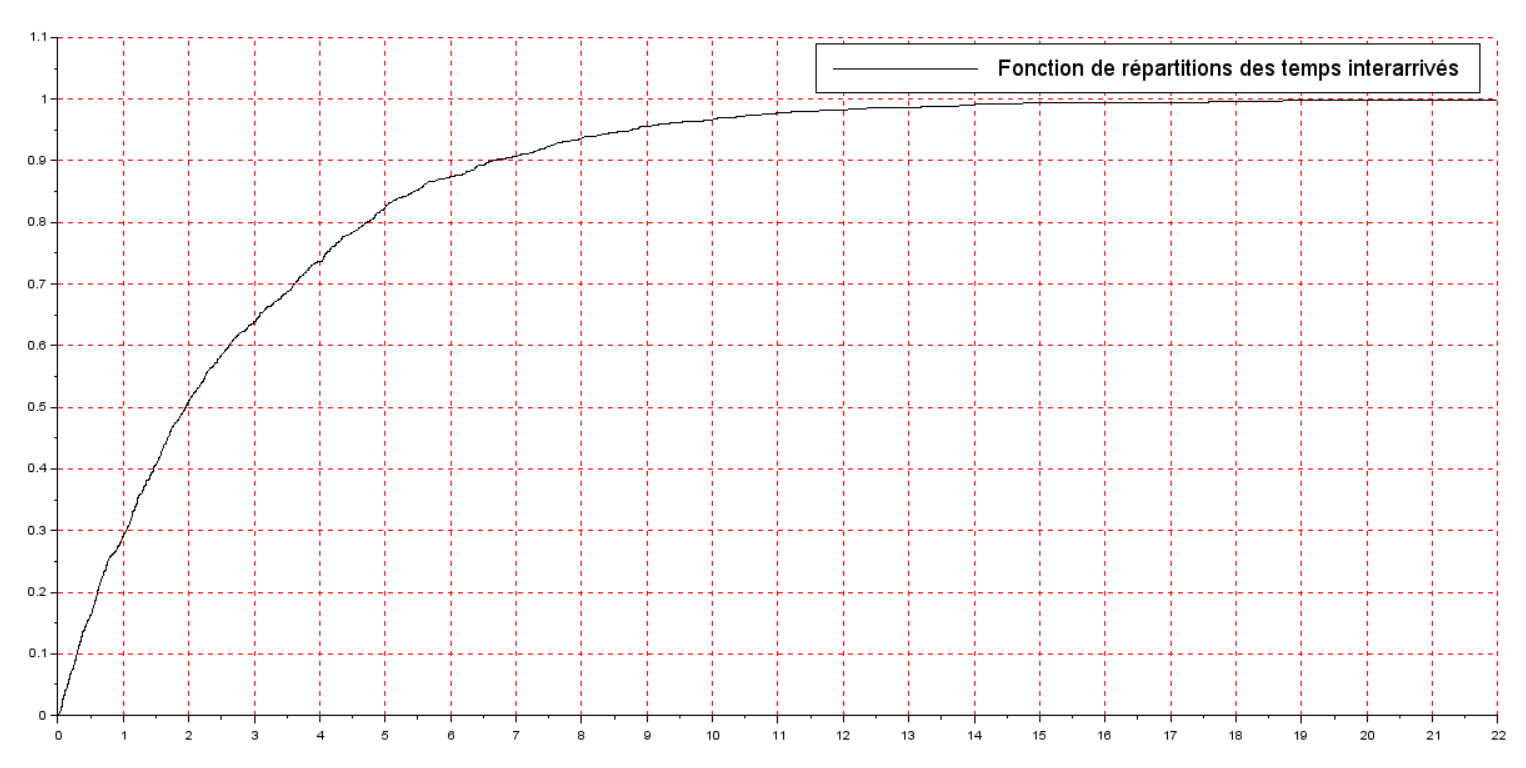
\includegraphics[width=425px]{img/repart.png}
\end{center}
\paragraph{}

\subsection{Histogramme}

\subsubsection{Histogramme avec classes isoamplitudes}
\begin{center}
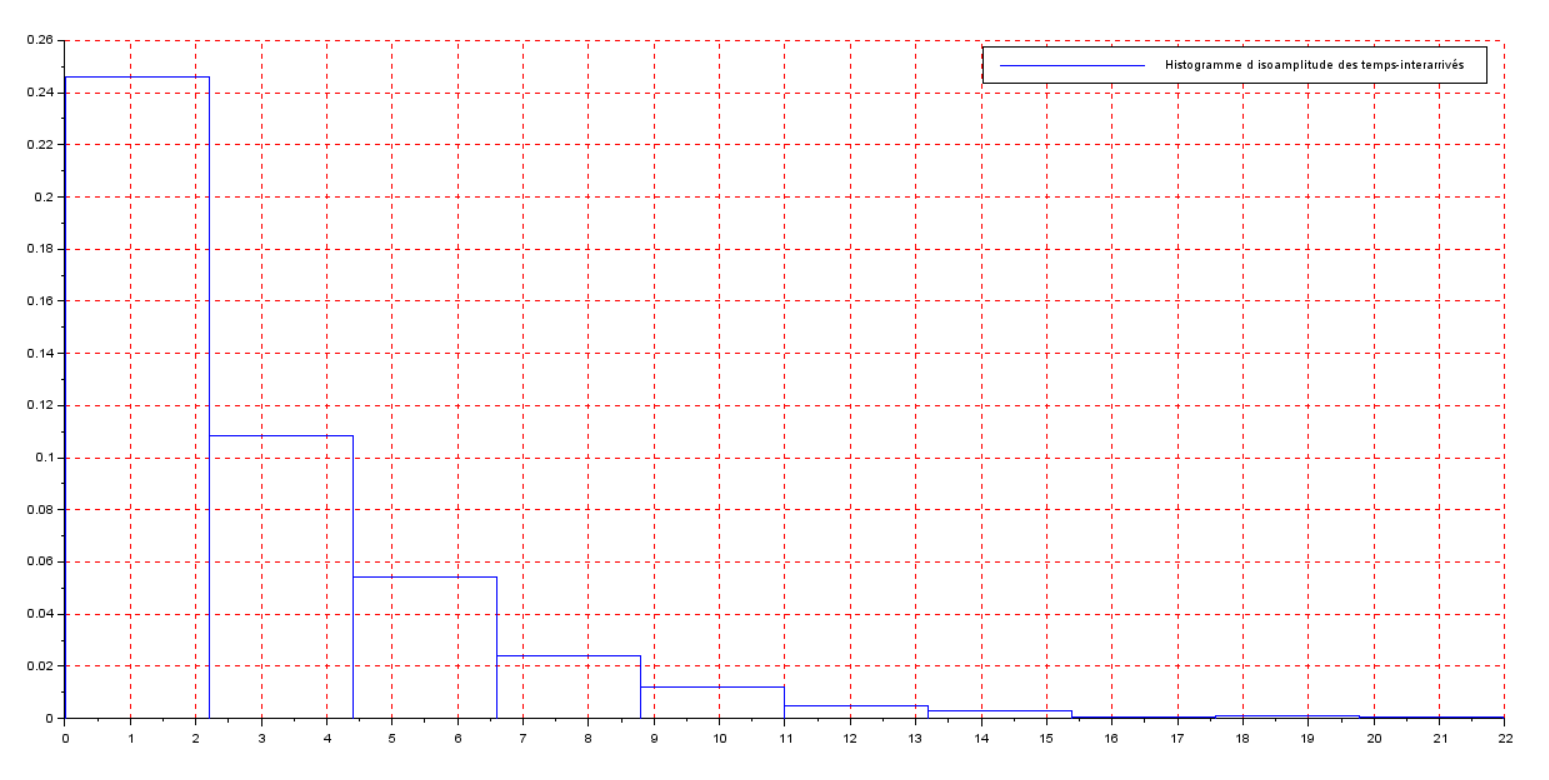
\includegraphics[width=425px]{img/H_isoa.png}
\end{center}
\paragraph{}

\subsubsection{Histogramme avec classes isofréquences}
\begin{center}
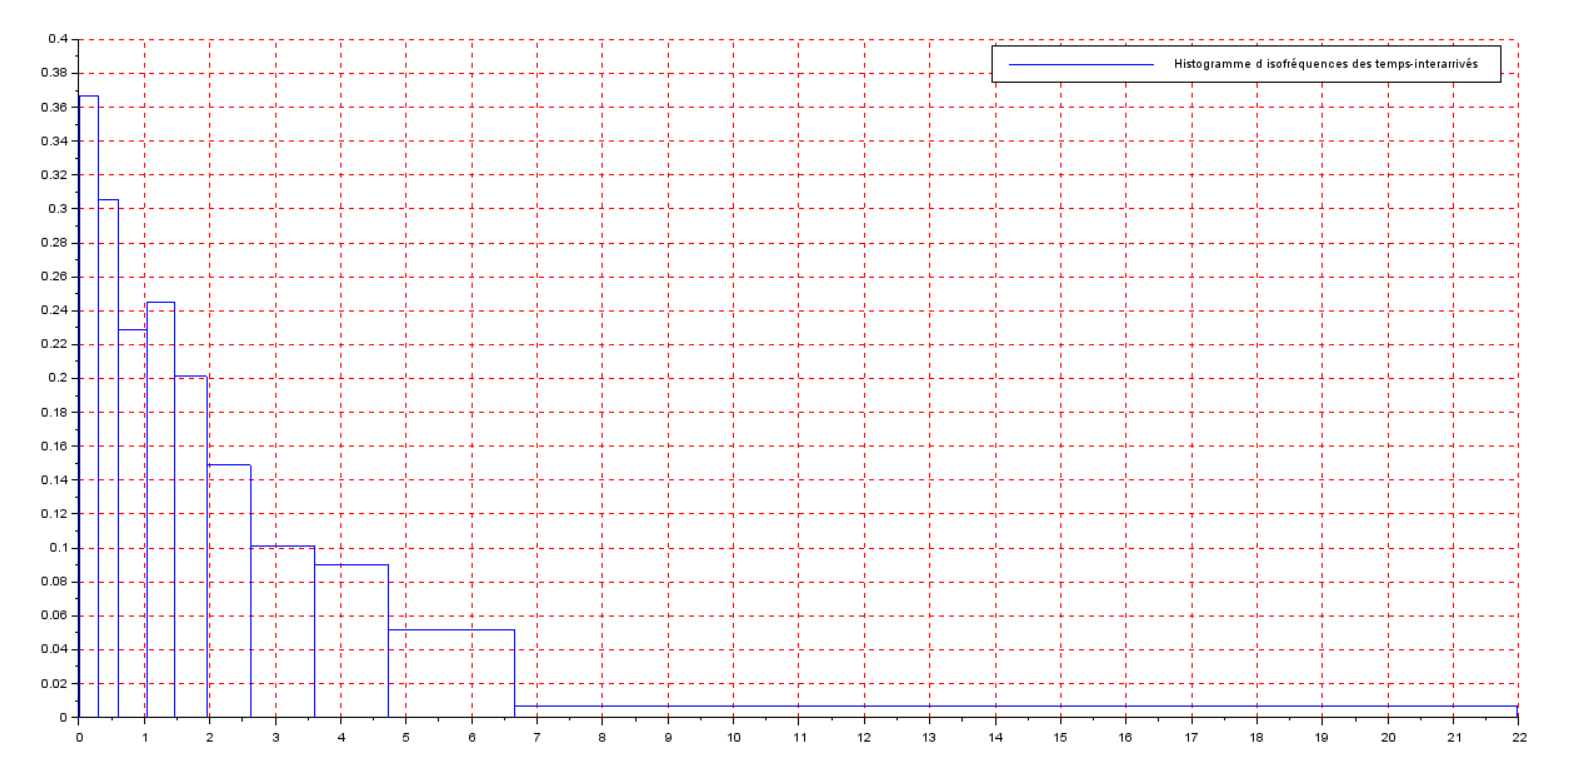
\includegraphics[width=425px]{img/H_isof.png}
\end{center}
\paragraph{}

\part{Etude statistique des temps de service}

\section{Indicateurs de position et de dispersion}

\begin{tabular}{|c|c|c|c|}
  \hline
  Indicateurs & Serveur 1 & Serveur 2 & Serveur 3 \\
  \hline
  Minimum & 0.01 & 0.04 & 0.01 \\
  Maximum & 134 & 88.9 & 68.6 \\
  Etendue & 134 & 88.8 & 68.6 \\
  \hline
  Moyenne & 15.5 & 10.6 & 6.27 \\
  Médiane & 11.5 & 6.82 & 4.35 \\
  \hline
  Q1 & 5.05 & 3.29 & 1.75 \\
  Q3 & 21.9 & 13.9 & 8.36 \\
  IQ & 16.8 & 10.6 & 6.61 \\
  \hline
  Ecart-Type & 15 & 11.3 & 6.85 \\
  Variance & 225 & 127 & 46.9 \\
  \hline
\end{tabular}

\section{Fonctions de répartition}

\subsection{Serveur 1}
\begin{center}
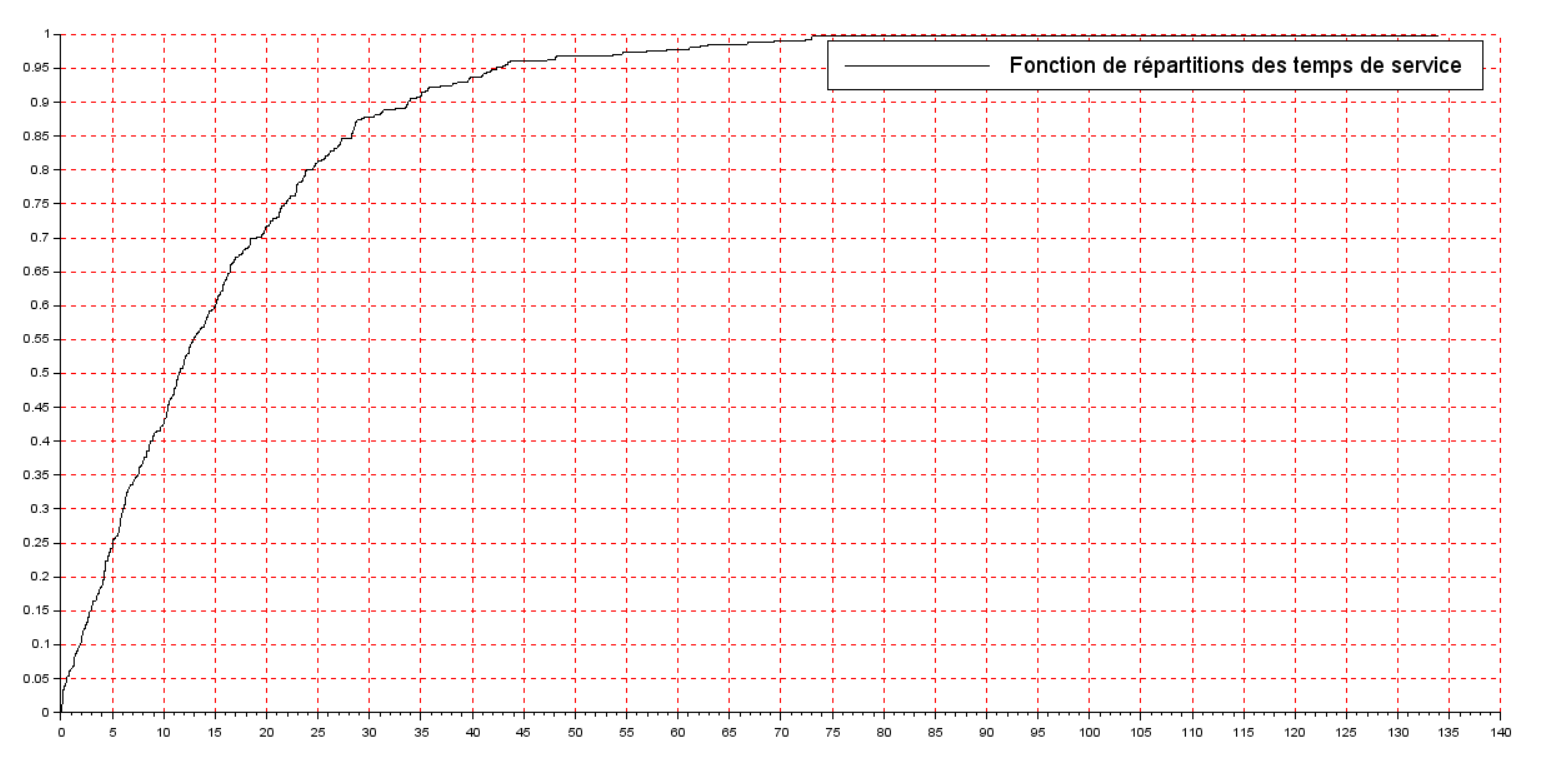
\includegraphics[width=425px]{img/S1_repart.png}
\end{center}
\paragraph{}

\subsection{Serveur 2}
\begin{center}
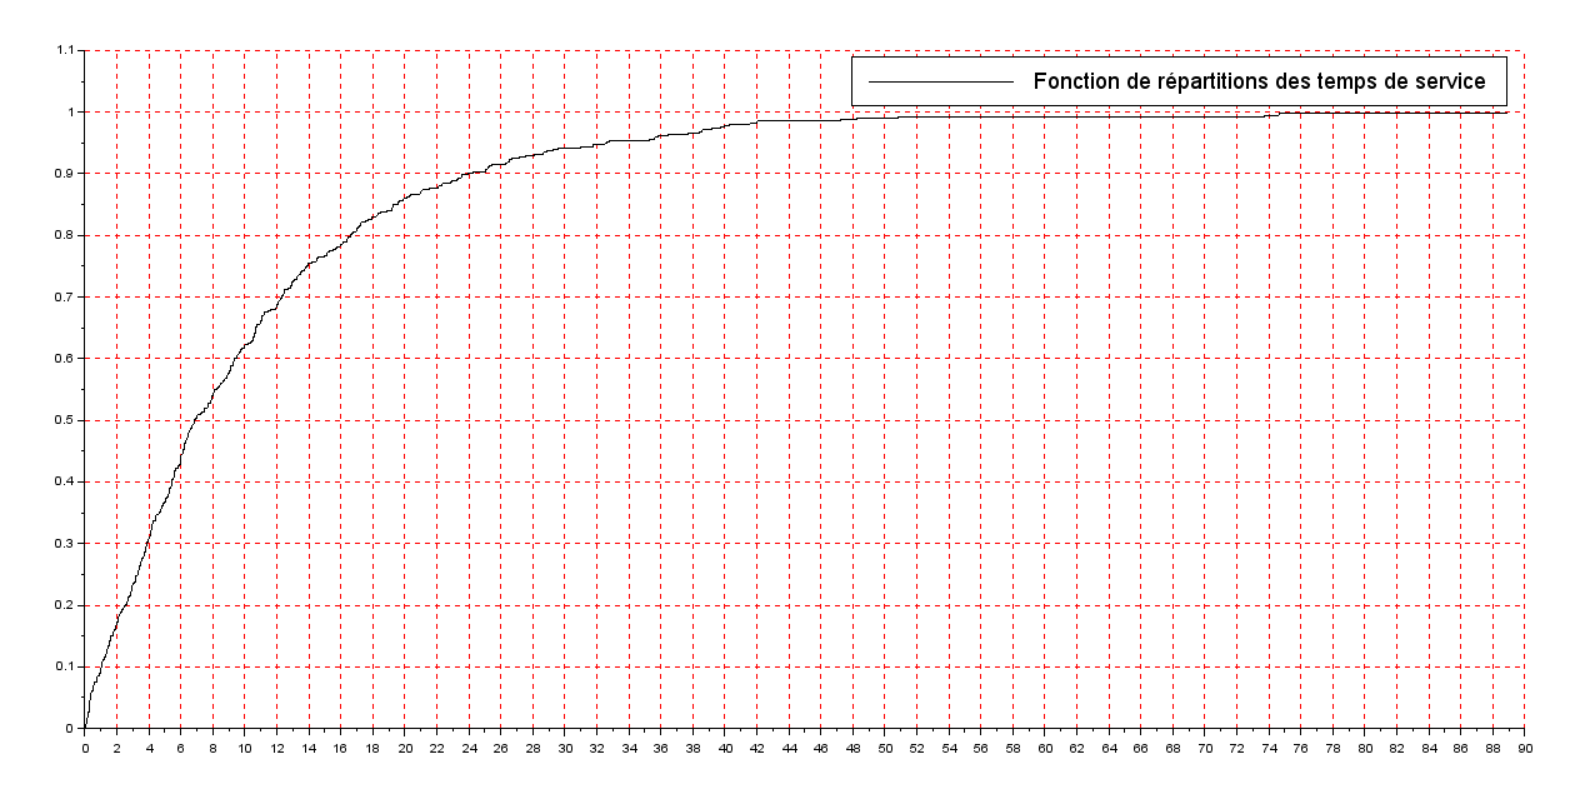
\includegraphics[width=425px]{img/S2_repart.png}
\end{center}
\paragraph{}

\subsection{Serveur 3}
\begin{center}
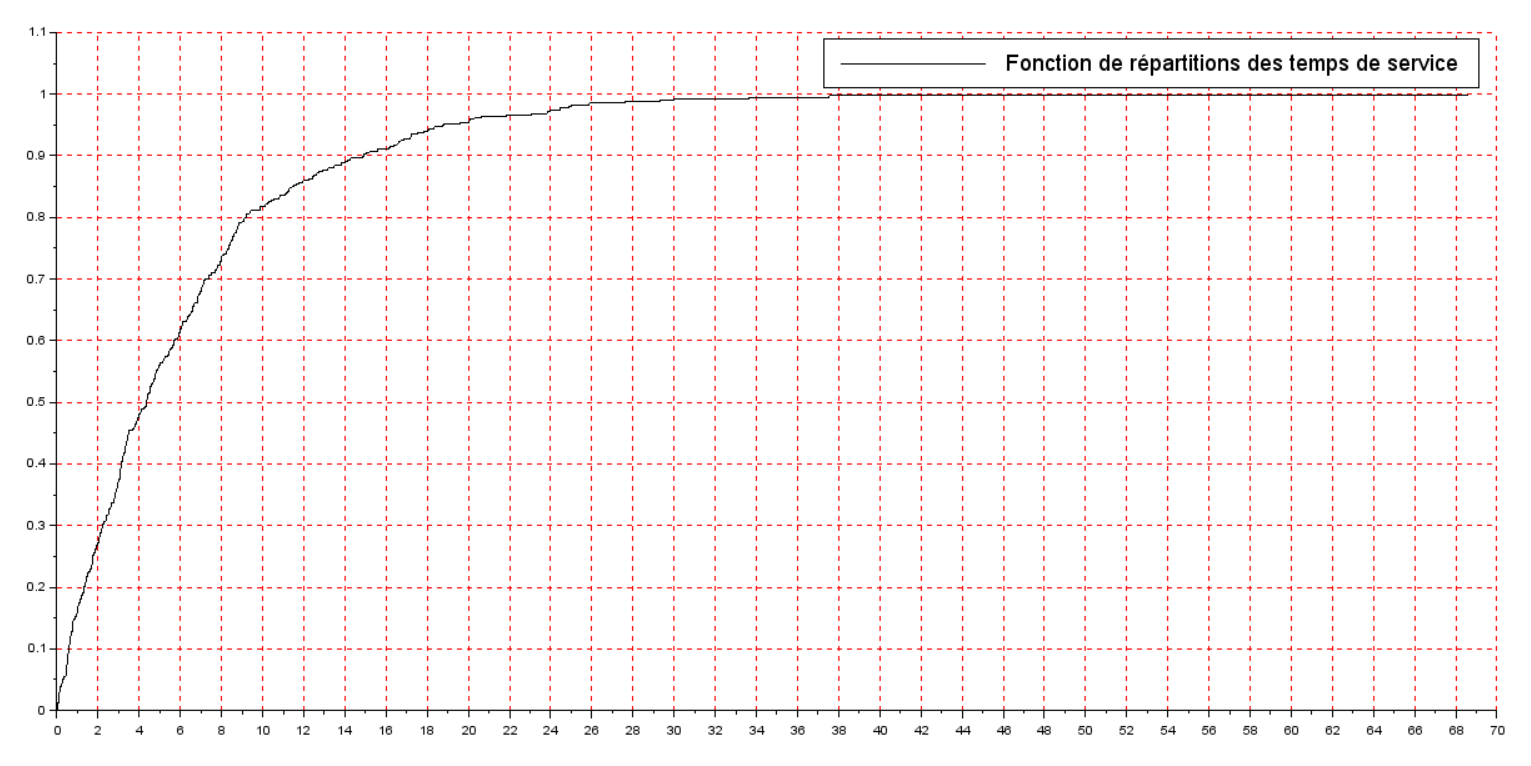
\includegraphics[width=425px]{img/S3_repart.png}
\end{center}
\paragraph{}

\section{Histogrammes}

\subsection{Serveur 1}
\begin{center}
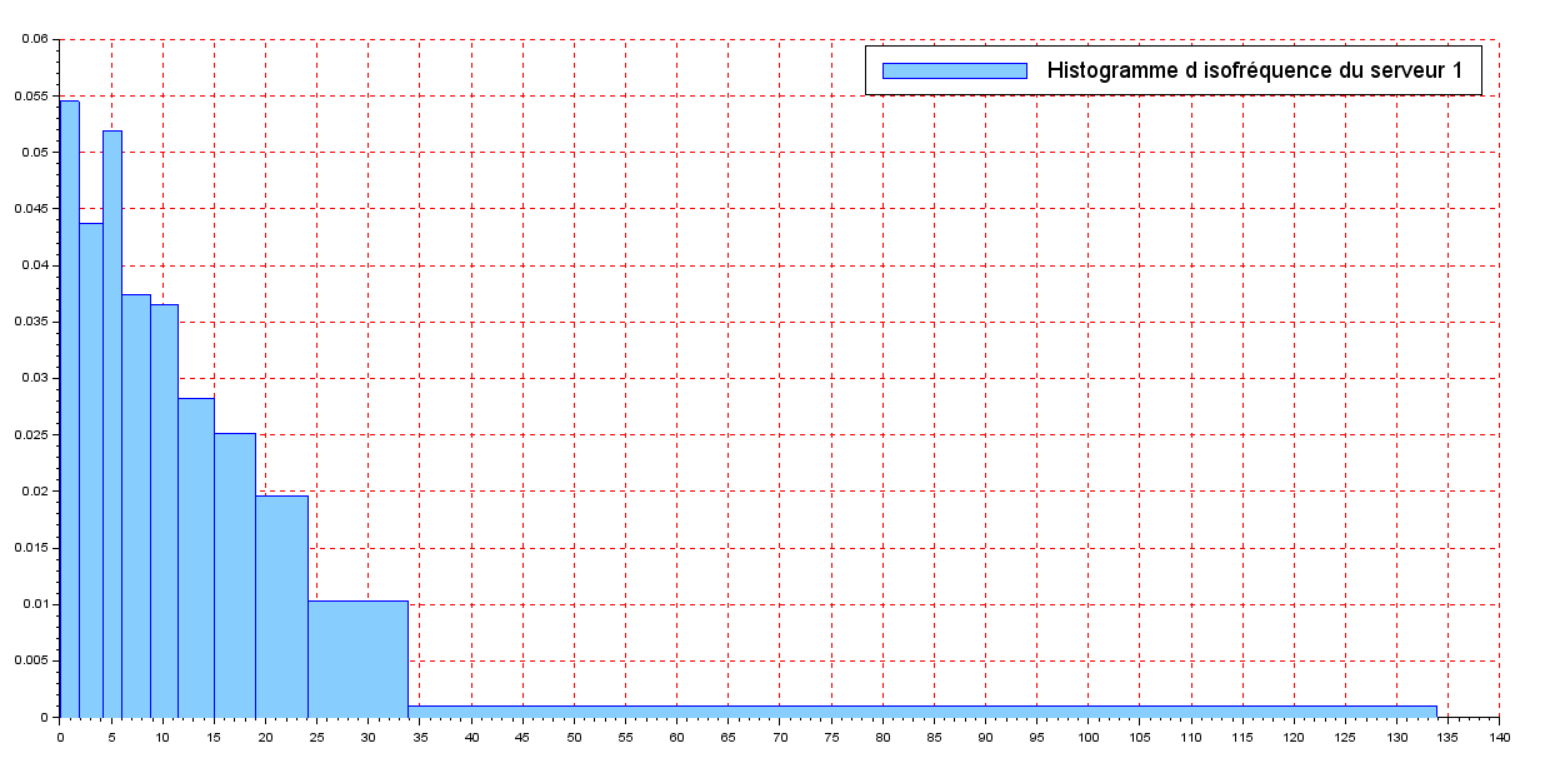
\includegraphics[width=425px]{img/S1_histo.png}
\end{center}
\paragraph{}

\subsection{Serveur 2}
\begin{center}
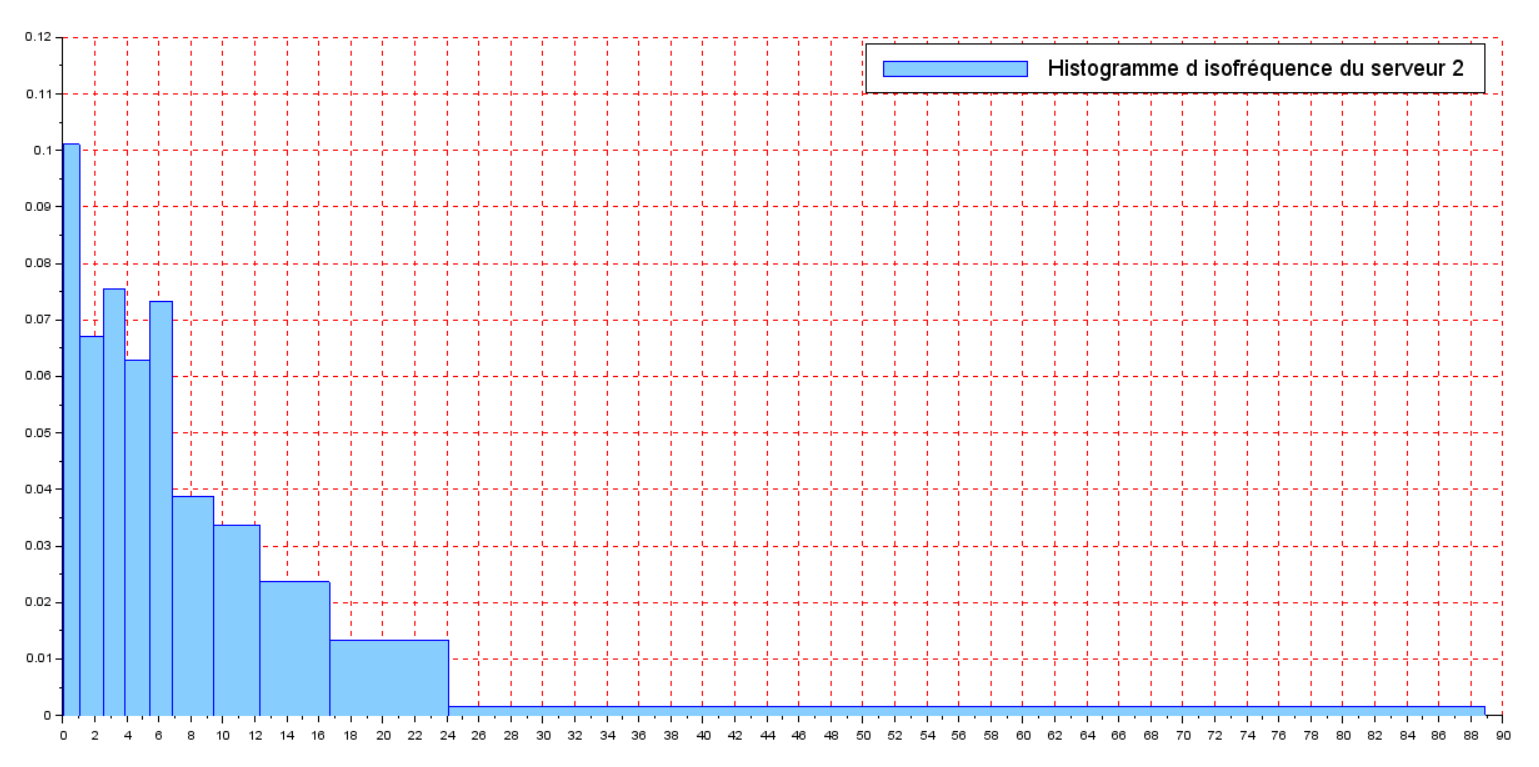
\includegraphics[width=425px]{img/S2_histo.png}
\end{center}
\paragraph{}

\subsection{Serveur 3}
\begin{center}
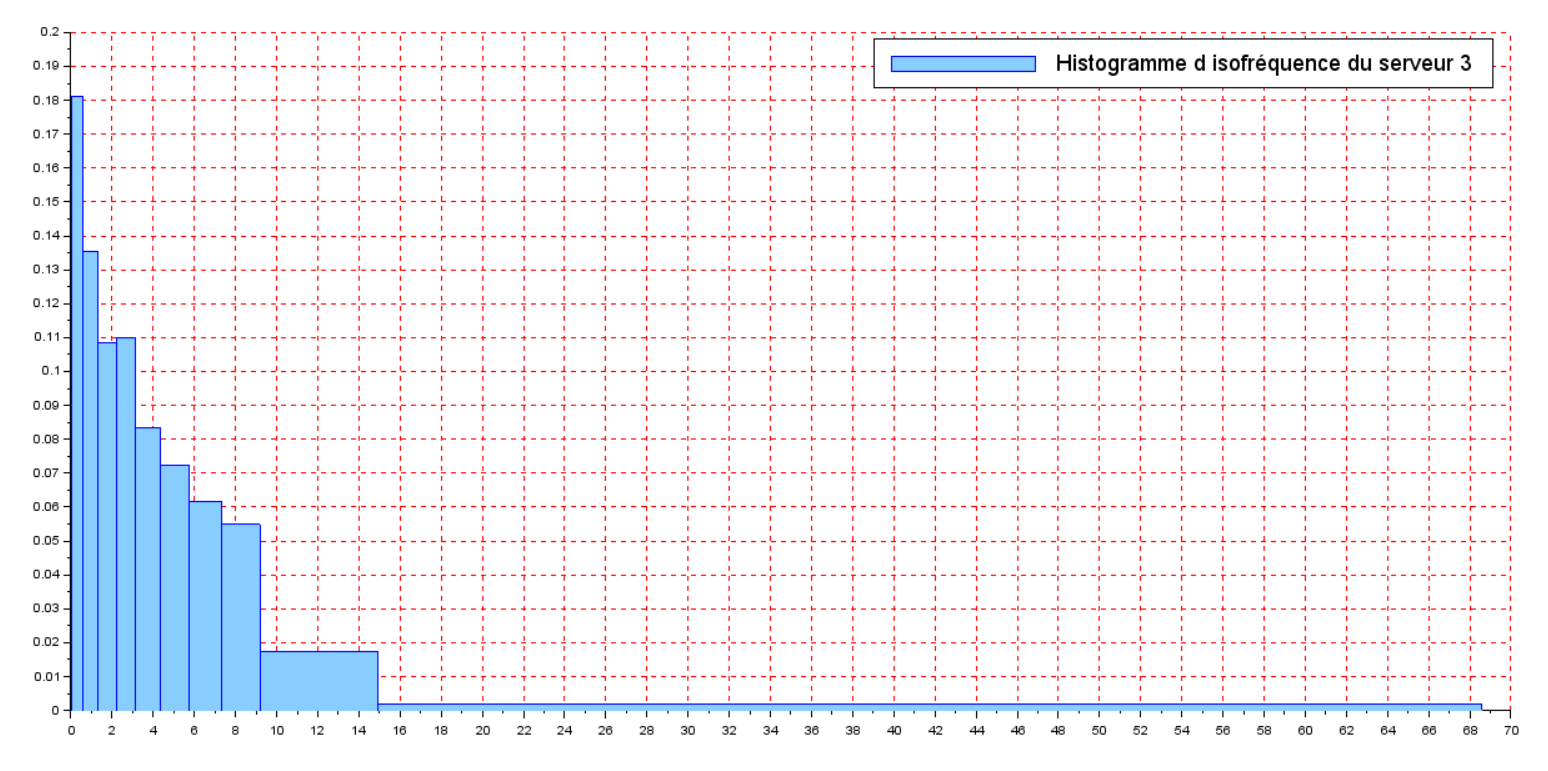
\includegraphics[width=425px]{img/S3_histo.png}
\end{center}
\paragraph{}

\part{Ajustement graphique à des lois mathématiques}

\section{Estimation des paramètres}

\subsection{Loi normale}
\paragraph{}
La loi normale $X \sim N(\mu,\sigma)$ s'exprime en fonction de l'esperance $\mu$ ainsi que de l'écart-type $\sigma$. On associe donc l'espérance à la moyenne des temps d'attentes/temps interarrivés.

\subsection{Loi uniforme}
\paragraph{}
La loi uniforme dépend de 2 paramètres : $a$ et $b$ qui correspondant à l'intervalle $[a,b]$ sur laquelle est définie la loi uniforme. On associe donc $a$ au minimum et $b$ au maximum des temps d'attentes/temps interarrivés.

\subsection{Loi exponentielle}
\paragraph{}
La loi exponentielle dépend d'un seul paramètre : $\lambda$.
Or on sait que pour une loi exponentielle $X$ :
\begin{align}
E(X) & =\frac{1}{\lambda} \\
V(X) & =\frac{1}{\lambda^2}
\intertext{Donc}
\lambda & =\frac{1}{E(X)} \\
\lambda & =\frac{1}{\sqrt{V(X)}} \\
&= \frac{1}{\sigma}
\end{align}
On en déduit déjà que pour qu'une la moyenne doit être égale à l'écart type pour que les temps de services soient les réalisations d'une loi exponentielle.

\section{Tous les serveurs}

\subsection{Superposition des fonctions de répartition}
\begin{center}
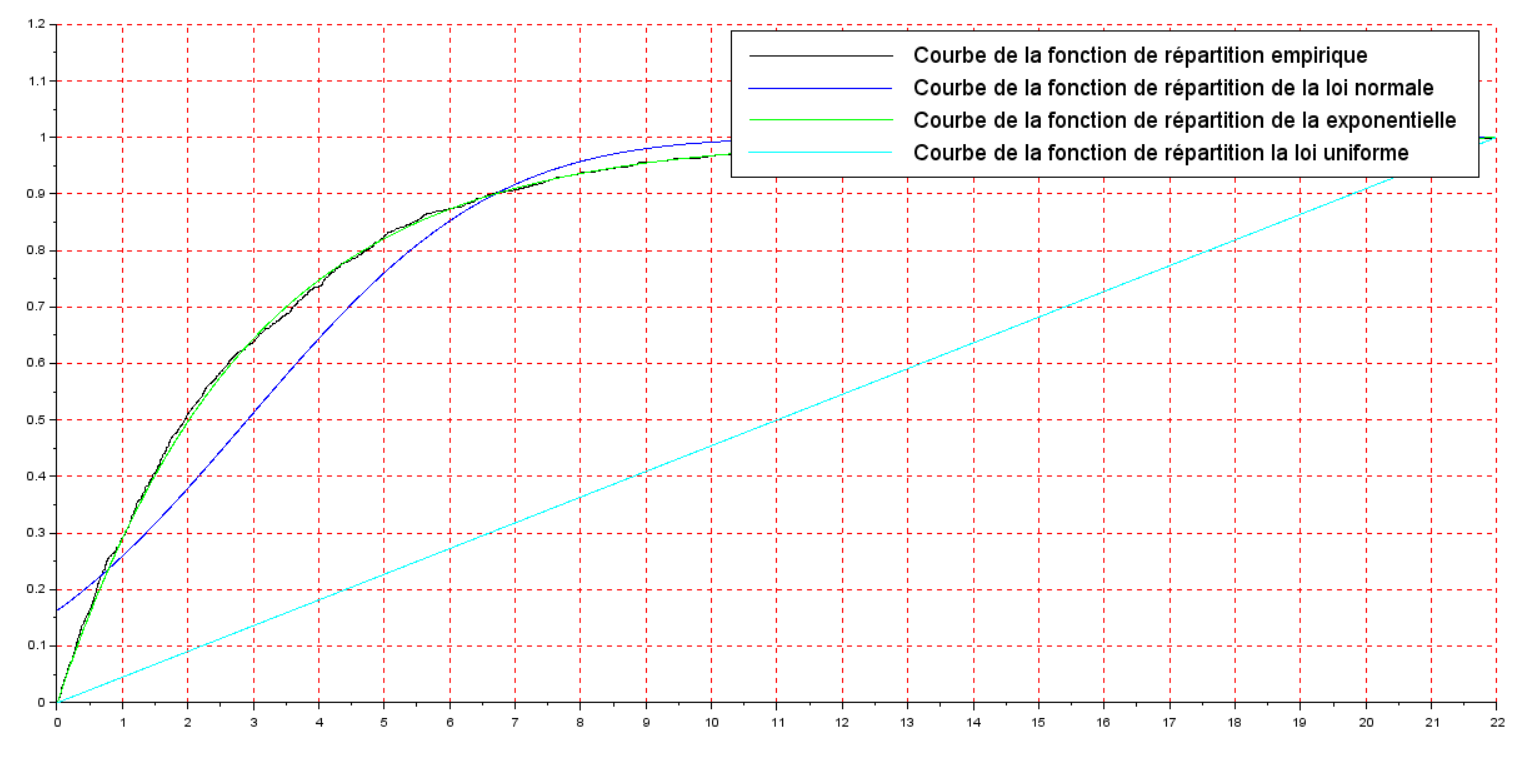
\includegraphics[width=300px]{img/repartitions.png}
\end{center}
\paragraph{}

\subsection{Superposition des fonctions de densité et de l'histogramme}
\begin{center}
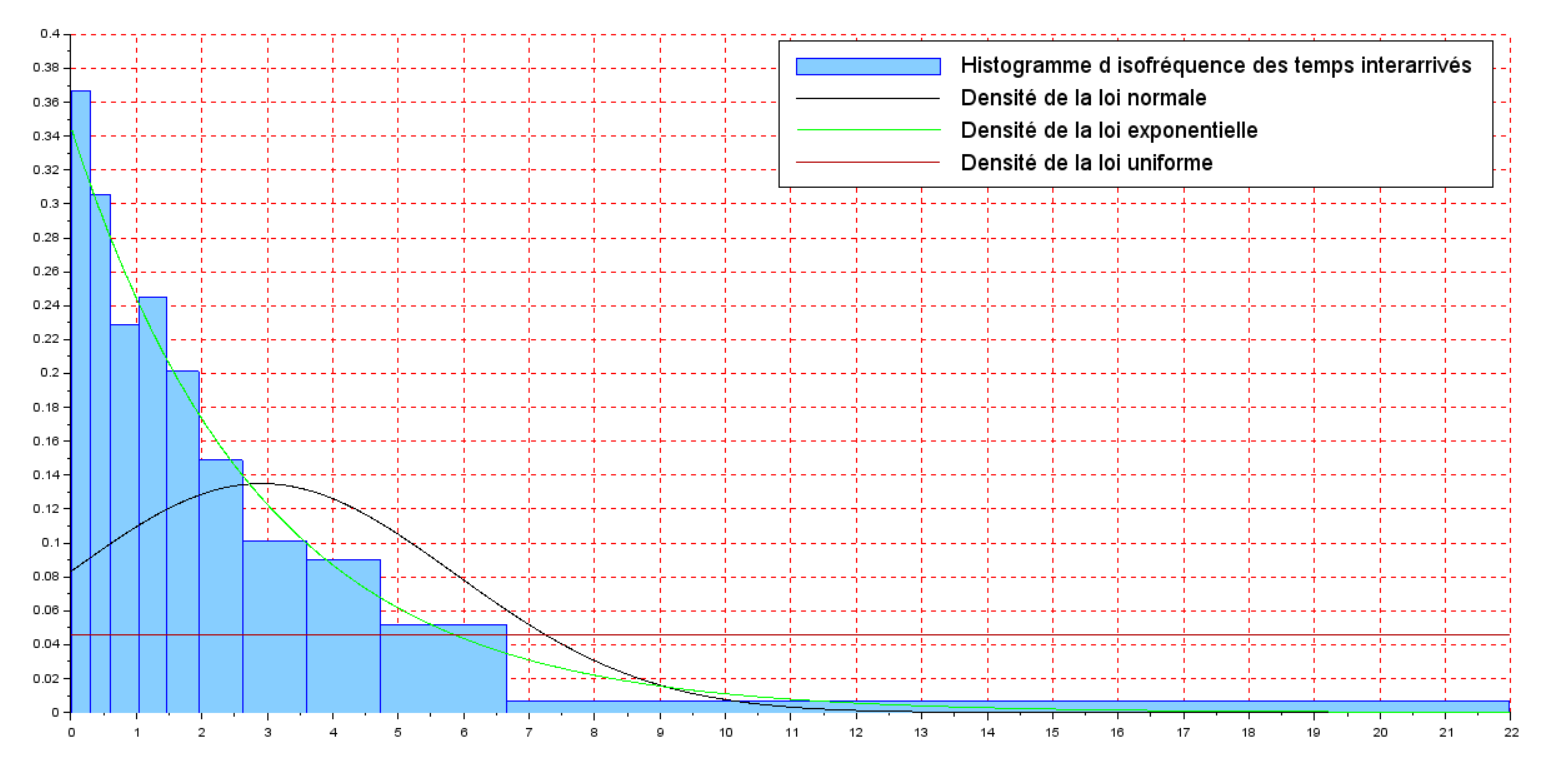
\includegraphics[width=300px]{img/densite.png}
\end{center}
\paragraph{}

\section{Serveur 1}

\subsection{Superposition des fonctions de répartition}
\begin{center}
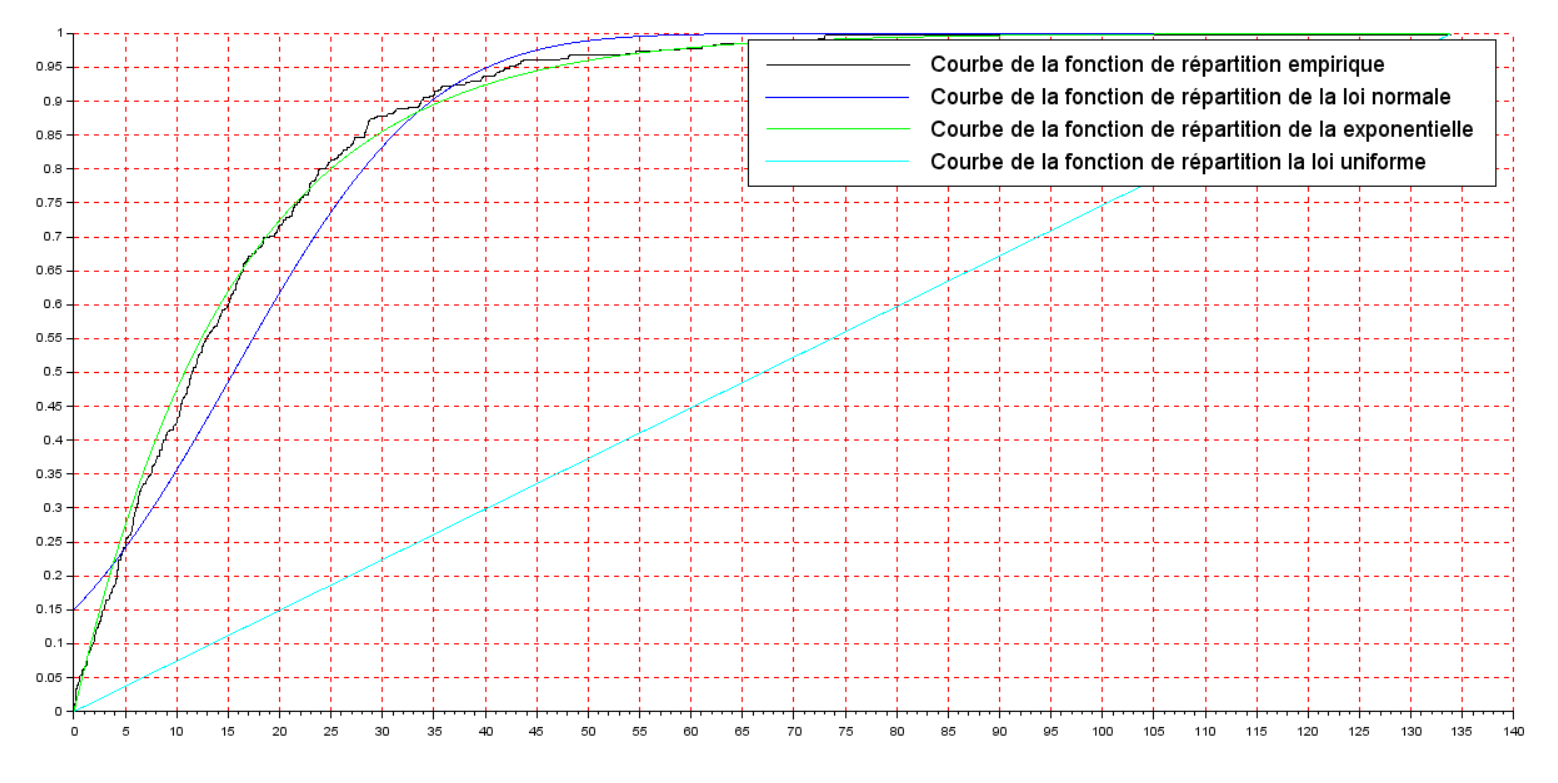
\includegraphics[width=300px]{img/S1_repartitions.png}
\end{center}
\paragraph{}

\subsection{Superposition des fonctions de densité et de l'histogramme}
\begin{center}
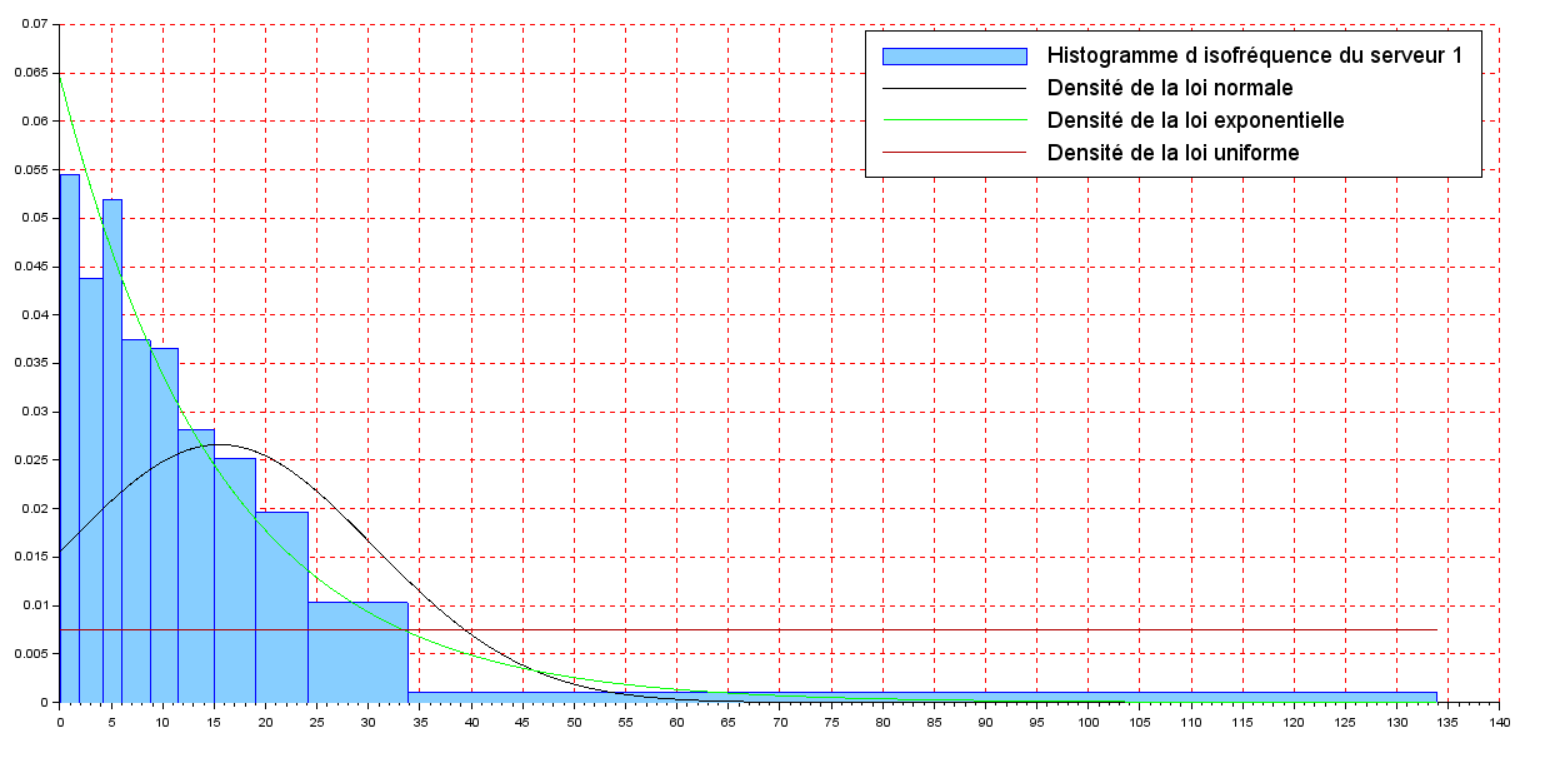
\includegraphics[width=300px]{img/S1_densite.png}
\end{center}
\paragraph{}

\section{Serveur 2}

\subsection{Superposition des fonctions de répartition}
\begin{center}
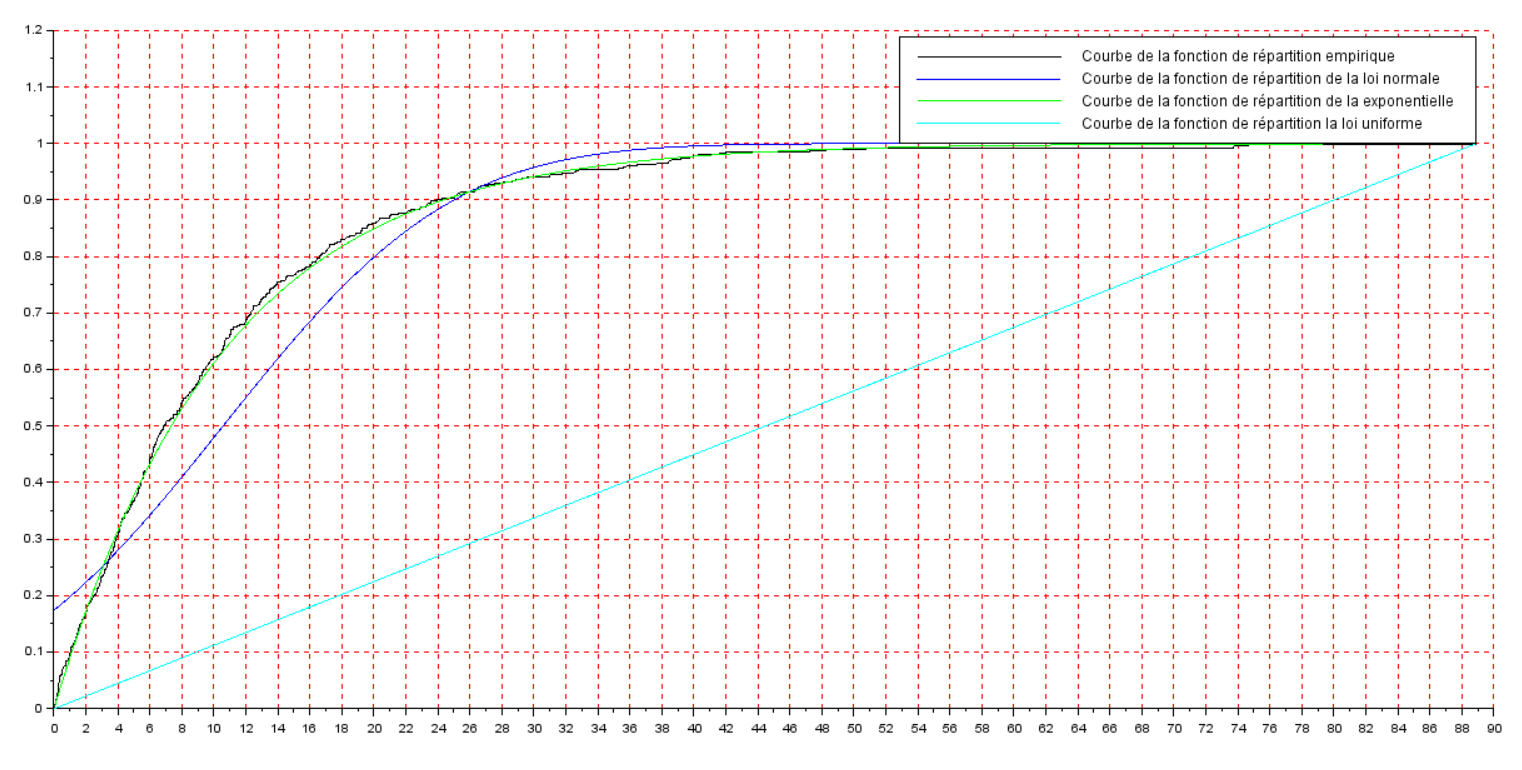
\includegraphics[width=300px]{img/S2_repartitions.png}
\end{center}
\paragraph{}

\subsection{Superposition des fonctions de densité et de l'histogramme}
\begin{center}
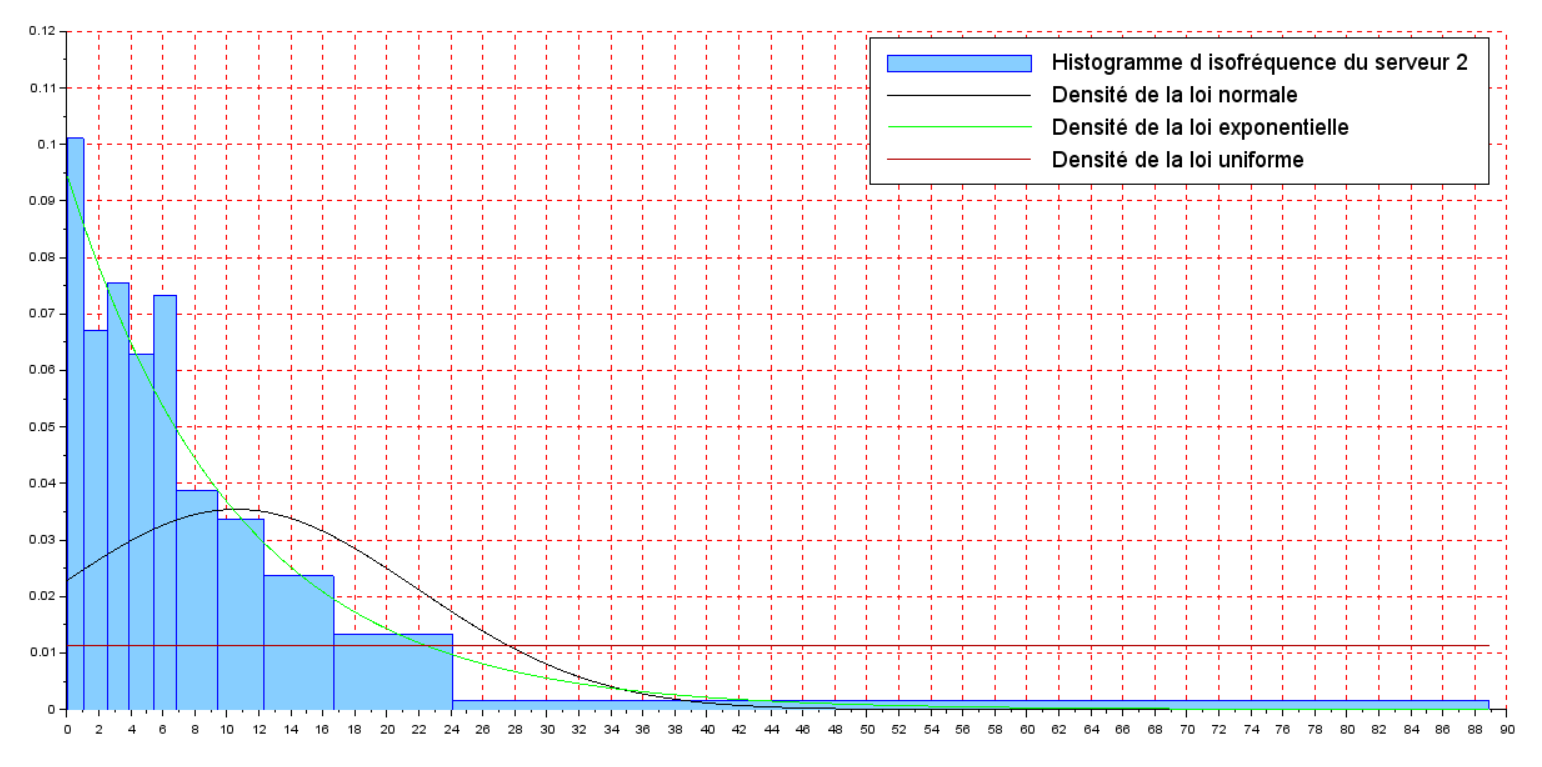
\includegraphics[width=300px]{img/S2_densite.png}
\end{center}
\paragraph{}

\section{Serveur 3}

\subsection{Superposition des fonctions de répartition}
\begin{center}
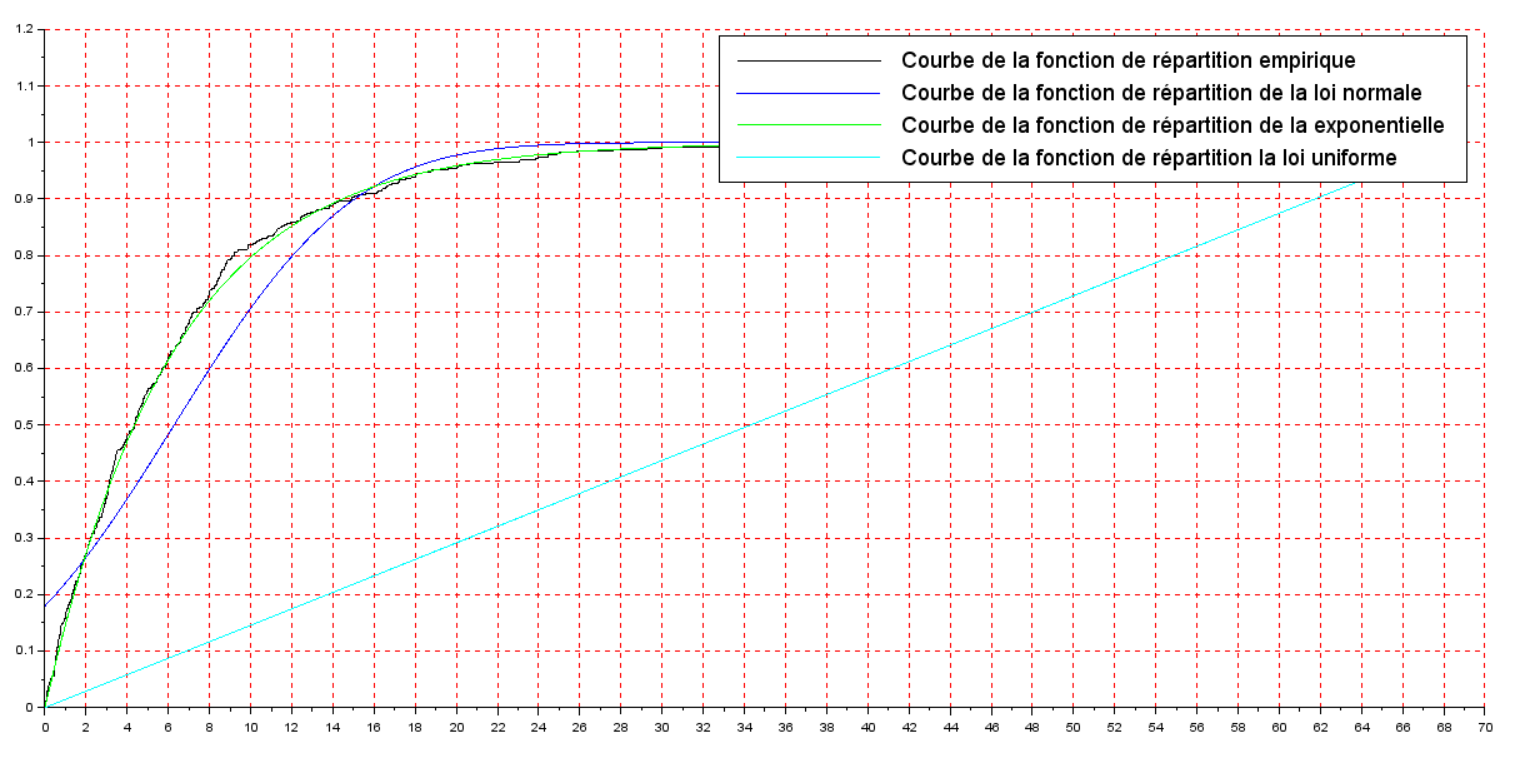
\includegraphics[width=300px]{img/S3_repartitions.png}
\end{center}
\paragraph{}

\subsection{Superposition des fonctions de densité et de l'histogramme}
\begin{center}
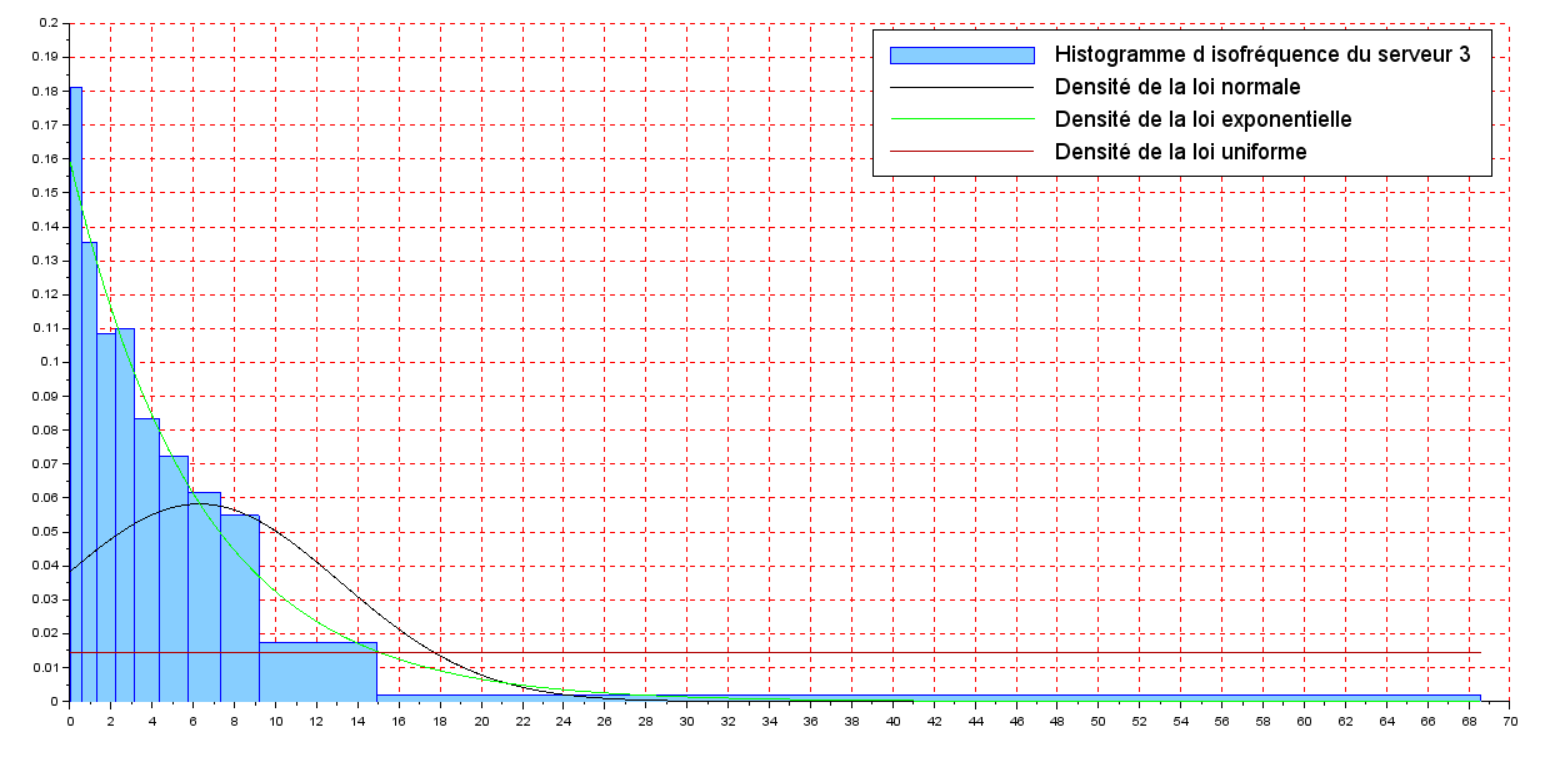
\includegraphics[width=300px]{img/S3_densite.png}
\end{center}
\paragraph{}

\newpage
\appendix

\section{Etude statistique des temps interarrivés}

\subsection{Indicateurs de position et de dispersion}
\begin{verbatim}
// Extraction des temps inter-arrivées
t_ia = data(2:$, 2) - data(1:1237, 2);

extremes = [min(t_ia), max(t_ia)] // calcul du min et du max
moyenne = mean(t_ia)  // calcul de la moyenne
mediane = perctl(t_ia,50) // calcul de la mediane

// calcul de la variance et de l'écart-type
v = variance(t_ia)
s = stdev(t_ia)

// calcul de l'étendue
etendue = extremes(2) - extremes(1)

Q1 = perctl(t_ia, 25) // premier quartile
Q3 = perctl(t_ia, 75) // troisième quartile
IQ = Q3(1) - Q1(1) // intervalle interquartile
\end{verbatim}

\subsection{Fonction de répartition}
\begin{verbatim}
// Extraction des temps inter-arrivées
t_ia = data(2:$, 2) - data(1:1237, 2);

tab = tabul(t_ia, 'i'); // construction du tableau des effectifs
tab(:,2) = tab(:,2)/length(t_ia); // calcul des fréquences
F = cumsum(tab(:,2)); // calcul des fréquences cumulées
plot2d2(tab(:,1),F)
legend("Fonction de répartitions des temps interarrivés")

// Définition des paramètres d'affichages
a=gca();
a.x_location = "origin";
a.grid=[5,5];

\end{verbatim}

\subsection{Histogramme}
\subsubsection{Histogramme avec classes isoamplitudes}
\begin{verbatim}
// Extraction des temps inter-arrivées
t_ia = data(2:$, 2) - data(1:1237, 2);

C = linspace(min(t_ia), max(t_ia), 11) // calcul des classes

histplot(C, t_ia, style=2) // dessine l'histogramme
legend("Histogramme d isoamplitude des temps-interarrivés")
\end{verbatim}
\subsubsection{Histogramme avec classes isofréquences}
\begin{verbatim}
// Extraction des temps inter-arrivées
t_ia = data(2:$, 2) - data(1:1237, 2);

deciles=perctl(t_ia,10:10:90) // Calcul des déciles
// Affectations d'isofréquences comme bornes de classes
for i=2:10
    ClassesDeciles(i)=deciles(i-1)
end
ClassesDeciles(1)=min(t_ia)
ClassesDeciles(11)=max(t_ia)

histplot(ClassesDeciles,t_ia,style=2) // dessine l'histogramme
legend("Histogramme d isofréquences des temps-interarrivés")
\end{verbatim}

\section{Etude statistique des temps de service}

\subsection{Indicateurs de position et de dispersion}

\subsubsection{Serveur 1}
\begin{verbatim}
// Extraction des temps de service
index_bool = ( data(:, 3) = 1 )
tabS1 = data(index_bool, :)
t_s1 = tabS1(1:$,4)

extremesS1 = [min(t_s1), max(t_s1)] // calcul du min et du max
moyenneS1 = mean(t_s1)  // calcul de la moyenne
medianeS1 = perctl(t_s1,50) // calcul de la mediane

// calcul de la variance et de l'écart-type
vS1 = variance(t_s1)
sS1 = stdev(t_s1)

// calcul de l'étendue
etendueS1 = extremesS1(2) - extremesS1(1)

Q1S1 = perctl(t_s1, 25) // premier quartile
Q3S1 = perctl(t_s1, 75) // troisième quartile
IQS1 = Q3S1(1) - Q1S1(1) // intervalle interquartile
\end{verbatim}

\subsubsection{Serveur 2}
\begin{verbatim}
// Extraction des temps de service
index_bool = ( data(:, 3) = 2 )
tabs2 = data(index_bool, :)
t_s2 = tabs2(1:$,4)

extremesS2 = [min(t_s2), max(t_s2)] // calcul du min et du max
moyenneS2 = mean(t_s2)  // calcul de la moyenne
medianeS2 = perctl(t_s2,50) // calcul de la mediane

// calcul de la variance et de l'écart-type
vS2 = variance(t_s2)
sS2 = stdev(t_s2)

// calcul de l'étendue
etendueS2 = extremesS2(2) - extremesS2(1)

Q1S2 = perctl(t_s2, 25) // premier quartile
Q3S2 = perctl(t_s2, 75) // troisième quartile
IQS2 = Q3S2(1) - Q1S2(1) // intervalle interquartile
\end{verbatim}

\subsubsection{Serveur 3}
\begin{verbatim}
// Extraction des temps de service
index_bool = ( data(:, 3) = 3 )
tabS3 = data(index_bool, :)
t_s3 = tabS3(1:$,4)

extremesS3 = [min(t_s3), max(t_s3)] // calcul du min et du max
moyenneS3 = mean(t_s3)  // calcul de la moyenne
medianeS3 = perctl(t_s3,50) // calcul de la mediane

// calcul de la variance et de l'écart-type
vS3 = variance(t_s3)
sS3 = stdev(t_s3)

// calcul de l'étendue
etendueS3 = extremesS3(2) - extremesS3(1)

Q1S3 = perctl(t_s3, 25) // premier quartile
Q3S3 = perctl(t_s3, 75) // troisième quartile
IQS3 = Q3S3(1) - Q1S3(1) // intervalle interquartile
\end{verbatim}

\subsection{Fonctions de repartitions}

\subsubsection{Serveur 1}
\begin{verbatim}
// Extraction des temps de service

index_bool = ( data(:, 3) == 1 )
tabS1 = data(index_bool, :)
t_s1 = tabS1(1:$,4);

tab = tabul(t_s1,'i')
tab(:,2) = tab(:,2)/length(t_s1)
F = cumsum(tab(:,2))

plot2d2(tab(:,1),F)
legend("Fonction de répartitions des temps de service")

// Définition des paramètres d'affichages
a=gca();
a.x_location = "origin";
a.grid=[5,5];
\end{verbatim}

\subsubsection{Serveur 2}
\begin{verbatim}
// Extraction des temps de service

index_bool = ( data(:, 3) == 2 )
tabS1 = data(index_bool, :)
t_s1 = tabS1(1:$,4);

tab = tabul(t_s1,'i')
tab(:,2) = tab(:,2)/length(t_s1)
F = cumsum(tab(:,2))

plot2d2(tab(:,1),F)
legend("Fonction de répartitions des temps de service")

// Définition des paramètres d'affichages
a=gca();
a.x_location = "origin";
a.grid=[5,5];
\end{verbatim}

\subsubsection{Serveur 3}
\begin{verbatim}
// Extraction des temps de service

index_bool = ( data(:, 3) == 3 )
tabS1 = data(index_bool, :)
t_s1 = tabS1(1:$,4);

tab = tabul(t_s1,'i')
tab(:,2) = tab(:,2)/length(t_s1)
F = cumsum(tab(:,2))

plot2d2(tab(:,1),F)
legend("Fonction de répartitions des temps de service")

// Définition des paramètres d'affichages
a=gca();
a.x_location = "origin";
a.grid=[5,5];
\end{verbatim}

\subsection{Histogrammes}

\subsubsection{Serveur 1}
\begin{verbatim}
// Extraction des temps de service
index_bool = ( data(:, 3) == 1 )
tabS1 = data(index_bool, :)
t_s1 = tabS1(1:$,4);

deciles=perctl(t_s1,10:10:90);
for i=2:10
    ClassesDeciles(i)=deciles(i-1)
end
ClassesDeciles(1)=min(t_s1)
ClassesDeciles(11)=max(t_s1)

histplot(ClassesDeciles,t_s1,style=2)
legend("Histogramme d isofréquence du serveur 1")

// Définition des paramètres d'affichages
a=gca();
a.x_location = "origin";
a.grid=[5,5];
\end{verbatim}

\subsubsection{Serveur 2}
\begin{verbatim}
// Extraction des temps de service
index_bool = ( data(:, 3) == 2 )
tabS2 = data(index_bool, :)
t_s2 = tabS2(1:$,4);

deciles=perctl(t_s2,10:10:90);
for i=2:10
    ClassesDeciles(i)=deciles(i-1)
end
ClassesDeciles(1)=min(t_s2)
ClassesDeciles(11)=max(t_s2)

histplot(ClassesDeciles,t_s2,style=2)
legend("Histogramme d isofréquence du serveur 2")

// Définition des paramètres d'affichages
a=gca();
a.x_location = "origin";
a.grid=[5,5];
\end{verbatim}

\subsubsection{Serveur 3}
\begin{verbatim}
// Extraction des temps de service
index_bool = ( data(:, 3) == 3 )
tabS3 = data(index_bool, :)
t_s3 = tabS3(1:$,4);

deciles=perctl(t_s3,10:10:90);
for i=2:10
    ClassesDeciles(i)=deciles(i-1)
end
ClassesDeciles(1)=min(t_s3)
ClassesDeciles(11)=max(t_s3)

histplot(ClassesDeciles,t_s3,style=2)
legend("Histogramme d isofréquence du serveur 3")

// Définition des paramètres d'affichages
a=gca();
a.x_location = "origin";
a.grid=[5,5];
\end{verbatim}

\section{Ajustement graphique à des lois mathématiques}

\subsection{Tous les serveurs}

\subsubsection{Superposition des fonctions de répartitions}
\begin{verbatim}
// Extraction des temps inter-arrivées
t_ia = data(2:$, 2) - data(1:1237, 2);

tab = tabul(t_ia, 'i'); // construction du tableau des effectifs
tab(:,2) = tab(:,2)/length(t_ia); // calcul des fréquences
F = cumsum(tab(:,2)); // calcul des fréquences cumulées
plot2d2(tab(:,1),F)
legend("Fonction de répartitions des temps interarrivés")

// Définition des paramètres d'affichages
a=gca();
a.x_location = "origin";
a.grid=[5,5];

// Répartition loi normale
a=min(t_ia):0.01:max(t_ia)
m=ones(a)*mean(t_ia)
s=ones(a)*stdev(t_ia)
[P,Q]=cdfnor("PQ",a,m,s)
plot2d2(a,P,style=2)

// Repartition loi exponentielle
lambda=1/mean(t_ia)
b=1-exp(-lambda*a)
plot2d2(a,b,style=3)

// Repartition loi uniforme
c=(a-min(t_ia))/(max(t_ia)-min(t_ia))
plot2d2(a,c,style=4)

legend("Courbe de la fonction de répartition empirique","Courbe de la fonction 
de répartition de la loi normale","Courbe de la fonction de répartition de la 
exponentielle","Courbe de la fonction de répartition la loi uniforme")
\end{verbatim}

\subsubsection{Superposition des fonctions de densité et de l'histogramme}
\begin{verbatim}
// Extraction des temps inter-arrivées
t_ia = data(2:$, 2) - data(1:1237, 2);

// Histogramme
deciles=perctl(t_ia,10:10:90);
for i=2:10
    ClassesDeciles(i)=deciles(i-1)
end
ClassesDeciles(1)=min(t_ia)
ClassesDeciles(11)=max(t_ia)
histplot(ClassesDeciles,t_ia,style=2)

// Densité de la loi normale
a=min(t_ia):0.01:max(t_ia)
m=mean(t_ia)
v=stdev(t_ia)
b=(1/(v*sqrt(2*%pi))*exp((-1/2)*((a-m)/v)^2))
plot2d2(a,b,style=1)

// Densité de la loi exponentielle
lambda=1/mean(t_ia)
b=lambda*exp(-lambda*a)
plot2d2(a,b,style=3)

// Densité de la loi uniforme
h=1/(max(t_ia)-min(t_ia))
b=ones(a)*h
plot2d2(a,b,style=20)

legend("Histogramme d isofréquence des temps interarrivés","Densité de la loi 
normale","Densité de la loi exponentielle","Densité de la loi uniforme")

// Définition des paramètres d'affichages
a=gca();
a.x_location = "origin";
a.grid=[5,5];
\end{verbatim}

\subsection{Serveur 1}

\subsubsection{Superposition des fonctions de répartitions}
\begin{verbatim}
// Extraction des temps de service

index_bool = ( data(:, 3) == 1 )
tabS1 = data(index_bool, :)
t_s1 = tabS1(1:$,4);

// Repartition empirique
tab = tabul(t_s1,'i')
tab(:,2) = tab(:,2)/length(t_s1)
F = cumsum(tab(:,2))

plot2d2(tab(:,1),F)

// Définition des paramètres d'affichages
a=gca();
a.x_location = "origin";
a.grid=[5,5];

// Répartition loi normale
a=min(t_s1):0.01:max(t_s1)
m=ones(a)*mean(t_s1)
s=ones(a)*stdev(t_s1)
[P,Q]=cdfnor("PQ",a,m,s)
plot2d2(a,P,style=2)

// Repartition loi exponentielle
lambda=1/mean(t_s1)
b=1-exp(-lambda*a)
plot2d2(a,b,style=3)

// Repartition loi uniforme
c=(a-min(t_s1))/(max(t_s1)-min(t_s1))
plot2d2(a,c,style=4)

legend("Courbe de la fonction de répartition empirique","Courbe de la fonction
de répartition de la loi normale","Courbe de la fonction de répartition de la 
exponentielle","Courbe de la fonction de répartition la loi uniforme")
\end{verbatim}

\subsubsection{Superposition des fonctions de densité et de l'histogramme}
\begin{verbatim}
// Extraction des temps de service
index_bool = ( data(:, 3) == 1 )
tabS1 = data(index_bool, :)
t_s1 = tabS1(1:$,4);

deciles=perctl(t_s1,10:10:90);
for i=2:10
    ClassesDeciles(i)=deciles(i-1)
end
ClassesDeciles(1)=min(t_s1)
ClassesDeciles(11)=max(t_s1)

histplot(ClassesDeciles,t_s1,style=2)

// Densité de la loi normale
a=min(t_s1):0.01:max(t_s1)
m=mean(t_s1)
v=stdev(t_s1)
b=(1/(v*sqrt(2*%pi))*exp((-1/2)*((a-m)/v)^2))
plot2d2(a,b,style=1)

// Densité de la loi exponentielle
lambda=1/mean(t_s1)
b=lambda*exp(-lambda*a)
plot2d2(a,b,style=3)

// Densité de la loi uniforme
h=1/(max(t_s1)-min(t_s1))
b=ones(a)*h
plot2d2(a,b,style=20)

legend("Histogramme d isofréquence du serveur 1","Densité de la loi 
normale","Densité de la loi exponentielle","Densité de la loi uniforme")

// Définition des paramètres d'affichages
a=gca();
a.x_location = "origin";
a.grid=[5,5];
\end{verbatim}

\subsection{Serveur 2}

\subsubsection{Superposition des fonctions de répartitions}
\begin{verbatim}
// Extraction des temps de service

index_bool = ( data(:, 3) == 2 )
tabS2 = data(index_bool, :)
t_s2 = tabS2(1:$,4);

// Repartition empirique
tab = tabul(t_s2,'i')
tab(:,2) = tab(:,2)/length(t_s2)
F = cumsum(tab(:,2))

plot2d2(tab(:,1),F)

// Définition des paramètres d'affichages
a=gca();
a.x_location = "origin";
a.grid=[5,5];

// Répartition loi normale
a=min(t_s2):0.01:max(t_s2)
m=ones(a)*mean(t_s2)
s=ones(a)*stdev(t_s2)
[P,Q]=cdfnor("PQ",a,m,s)
plot2d2(a,P,style=2)

// Repartition loi exponentielle
lambda=1/mean(t_s2)
b=1-exp(-lambda*a)
plot2d2(a,b,style=3)

// Repartition loi uniforme
c=(a-min(t_s2))/(max(t_s2)-min(t_s2))
plot2d2(a,c,style=4)

legend("Courbe de la fonction de répartition empirique","Courbe de la fonction 
de répartition de la loi normale","Courbe de la fonction de répartition de la 
exponentielle","Courbe de la fonction de répartition la loi uniforme")
\end{verbatim}

\subsubsection{Superposition des fonctions de densité et de l'histogramme}
\begin{verbatim}
// Extraction des temps de service
index_bool = ( data(:, 3) == 2 )
tabS2 = data(index_bool, :)
t_s2 = tabS2(1:$,4);

deciles=perctl(t_s2,10:10:90);
for i=2:10
    ClassesDeciles(i)=deciles(i-1)
end
ClassesDeciles(1)=min(t_s2)
ClassesDeciles(11)=max(t_s2)

histplot(ClassesDeciles,t_s2,style=2)

// Densité de la loi normale
a=min(t_s2):0.01:max(t_s2)
m=mean(t_s2)
v=stdev(t_s2)
b=(1/(v*sqrt(2*%pi))*exp((-1/2)*((a-m)/v)^2))
plot2d2(a,b,style=1)

// Densité de la loi exponentielle
lambda=1/mean(t_s2)
b=lambda*exp(-lambda*a)
plot2d2(a,b,style=3)

// Densité de la loi uniforme
h=1/(max(t_s2)-min(t_s2))
b=ones(a)*h
plot2d2(a,b,style=20)

legend("Histogramme d isofréquence du serveur 2","Densité de la loi 
normale","Densité de la loi exponentielle","Densité de la loi uniforme")

// Définition des paramètres d'affichages
a=gca();
a.x_location = "origin";
a.grid=[5,5];
\end{verbatim}

\subsection{Serveur 3}

\subsubsection{Superposition des fonctions de répartitions}
\begin{verbatim}
// Extraction des temps de service

index_bool = ( data(:, 3) == 3 )
tabS3 = data(index_bool, :)
t_s3 = tabS3(1:$,4);

// Repartition empirique
tab = tabul(t_s3,'i')
tab(:,2) = tab(:,2)/length(t_s3)
F = cumsum(tab(:,2))

plot2d2(tab(:,1),F)

// Définition des paramètres d'affichages
a=gca();
a.x_location = "origin";
a.grid=[5,5];

// Répartition loi normale
a=min(t_s3):0.01:max(t_s3)
m=ones(a)*mean(t_s3)
s=ones(a)*stdev(t_s3)
[P,Q]=cdfnor("PQ",a,m,s)
plot2d2(a,P,style=2)

// Repartition loi exponentielle
lambda=1/mean(t_s3)
b=1-exp(-lambda*a)
plot2d2(a,b,style=3)

// Repartition loi uniforme
c=(a-min(t_s3))/(max(t_s3)-min(t_s3))
plot2d2(a,c,style=4)

legend("Courbe de la fonction de répartition empirique","Courbe de la fonction 
de répartition de la loi normale","Courbe de la fonction de répartition de la 
exponentielle","Courbe de la fonction de répartition la loi uniforme")
\end{verbatim}

\subsubsection{Superposition des fonctions de densité et de l'histogramme}
\begin{verbatim}
// Extraction des temps de service
index_bool = ( data(:, 3) == 3 )
tabS3 = data(index_bool, :)
t_s3 = tabS3(1:$,4);

deciles=perctl(t_s3,10:10:90);
for i=2:10
    ClassesDeciles(i)=deciles(i-1)
end
ClassesDeciles(1)=min(t_s3)
ClassesDeciles(11)=max(t_s3)

histplot(ClassesDeciles,t_s3,style=2)

// Densité de la loi normale
a=min(t_s3):0.01:max(t_s3)
m=mean(t_s3)
v=stdev(t_s3)
b=(1/(v*sqrt(2*%pi))*exp((-1/2)*((a-m)/v)^2))
plot2d2(a,b,style=1)

// Densité de la loi exponentielle
lambda=1/mean(t_s3)
b=lambda*exp(-lambda*a)
plot2d2(a,b,style=3)

// Densité de la loi uniforme
h=1/(max(t_s3)-min(t_s3))
b=ones(a)*h
plot2d2(a,b,style=20)

legend("Histogramme d isofréquence du serveur 3","Densité de la loi
normale","Densité de la loi exponentielle","Densité de la loi uniforme")

// Définition des paramètres d'affichages
a=gca();
a.x_location = "origin";
a.grid=[5,5];


\end{verbatim}


%----------------------------------

\begin{verbatim}
\end{verbatim}

\end{document}